% ============================================
\section{Models and regressions}
% ============================================


\begin{frame}[t]{ML model}

    \textbf{We built a simple empirical mathematical model
        that captures the saturating nature of nominal wage growth with professional experience
        (driven by raises, promotions, etc.):}

    \pause

    \begin{equation}
    k(x) = 1 + \alpha (1 - e^{-\beta x})
    \end{equation}
    \pause
    \\[.5cm]
    \centering
    $x$ --- years of professional experience
    \pause
    $\textrm{salary} \pause = \textrm{junior salary} \pause \cdot k(x)$
\end{frame}

\begin{frame}[plain]
    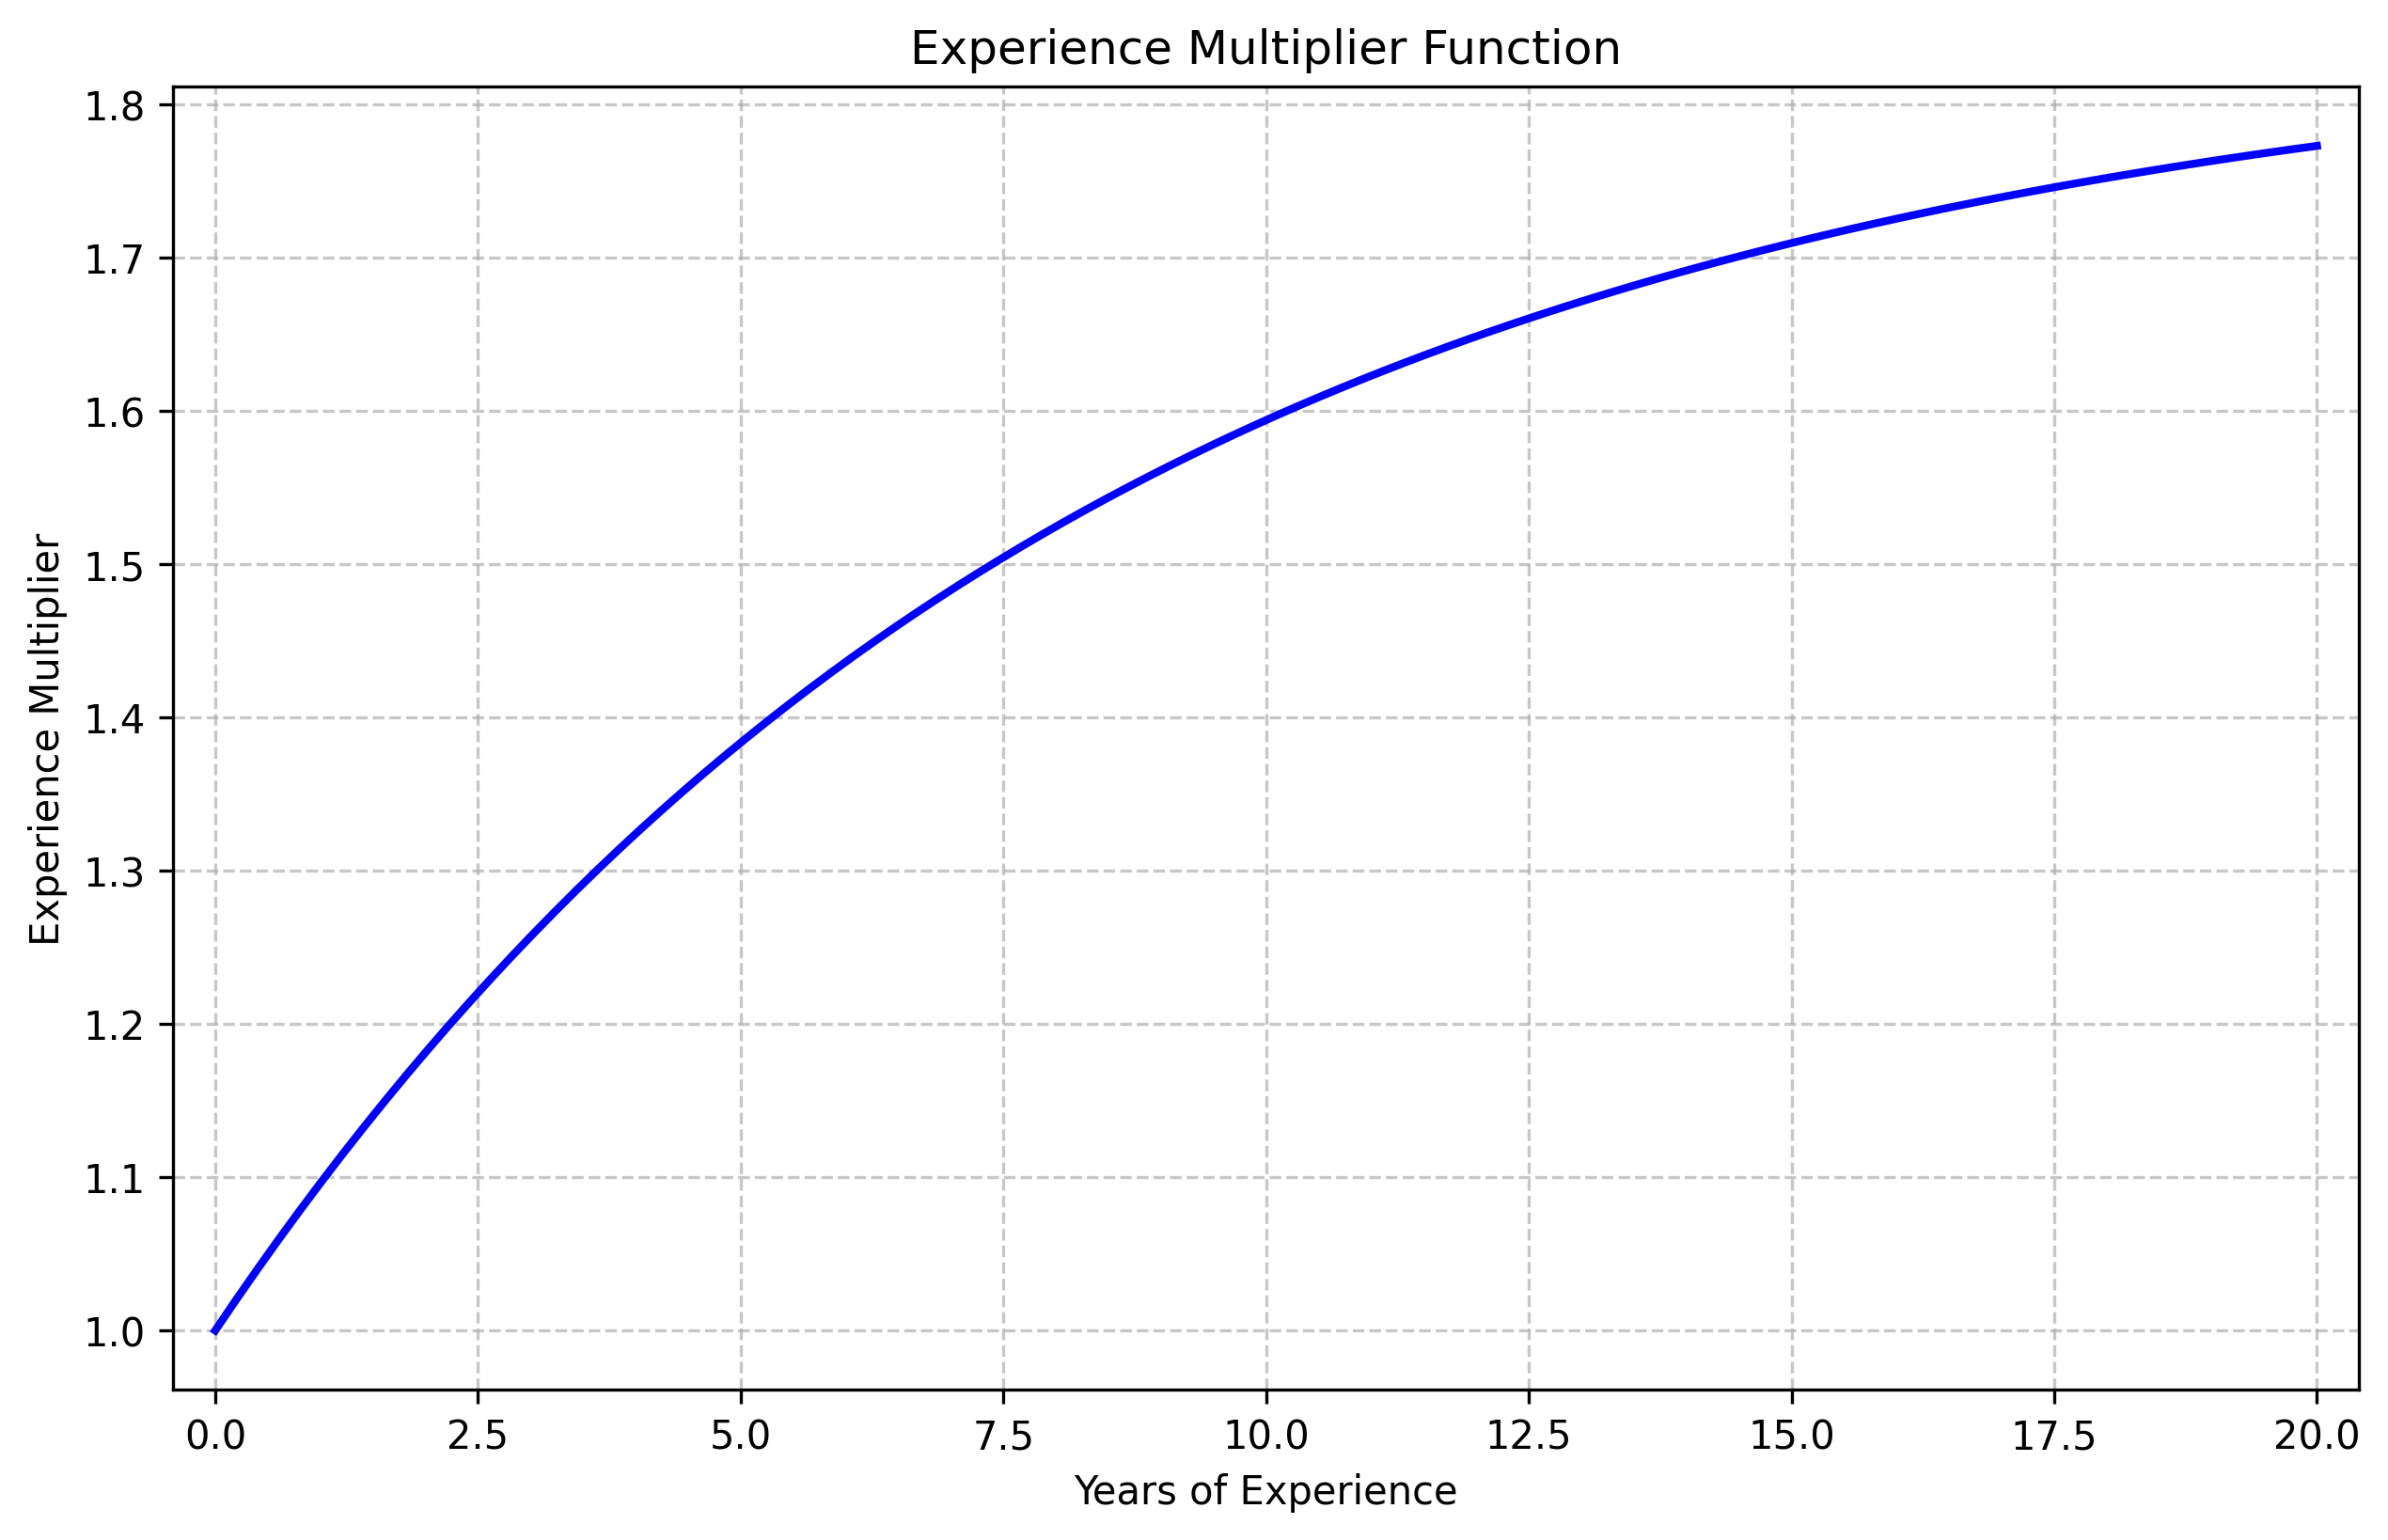
\includegraphics[width=.8\textwidth]{img/experience_multiplier}
\end{frame}

\begin{frame}[t]{Regressions for real‑world data}
\centering
\begin{tabular}{cc}
    \pause
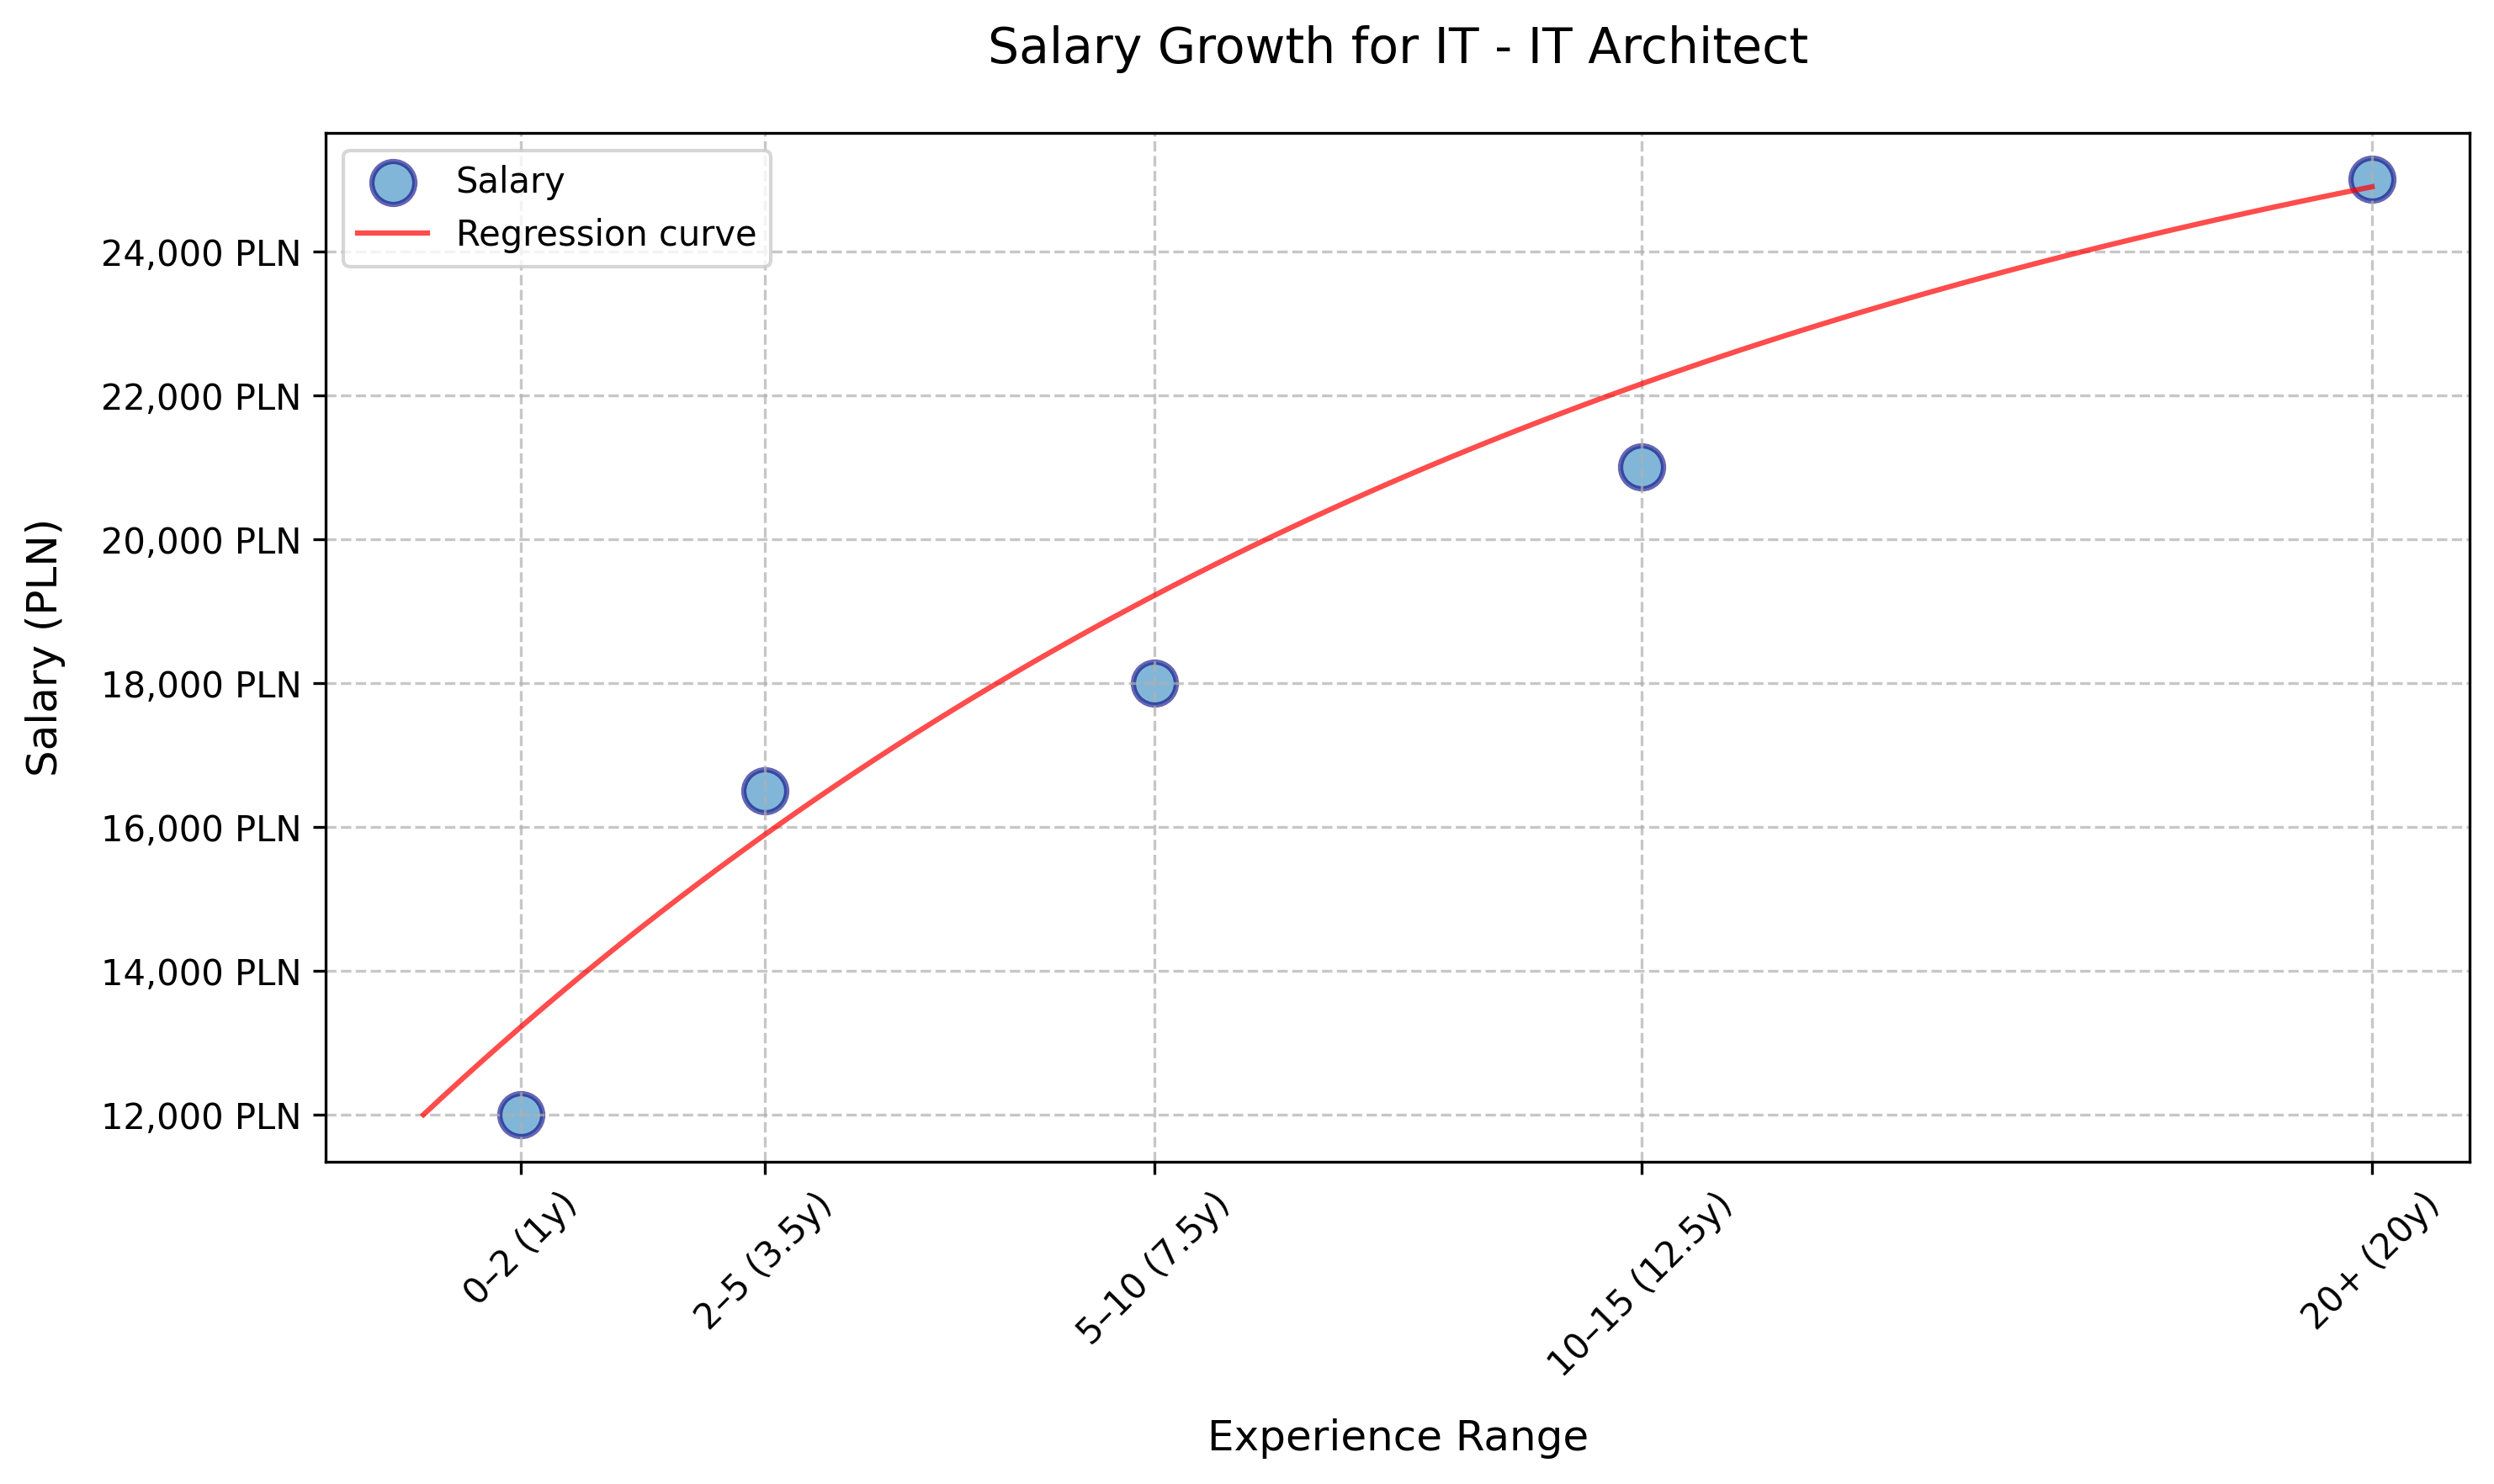
\includegraphics[width=0.45\linewidth]{img/salary_progression2} &
    \pause
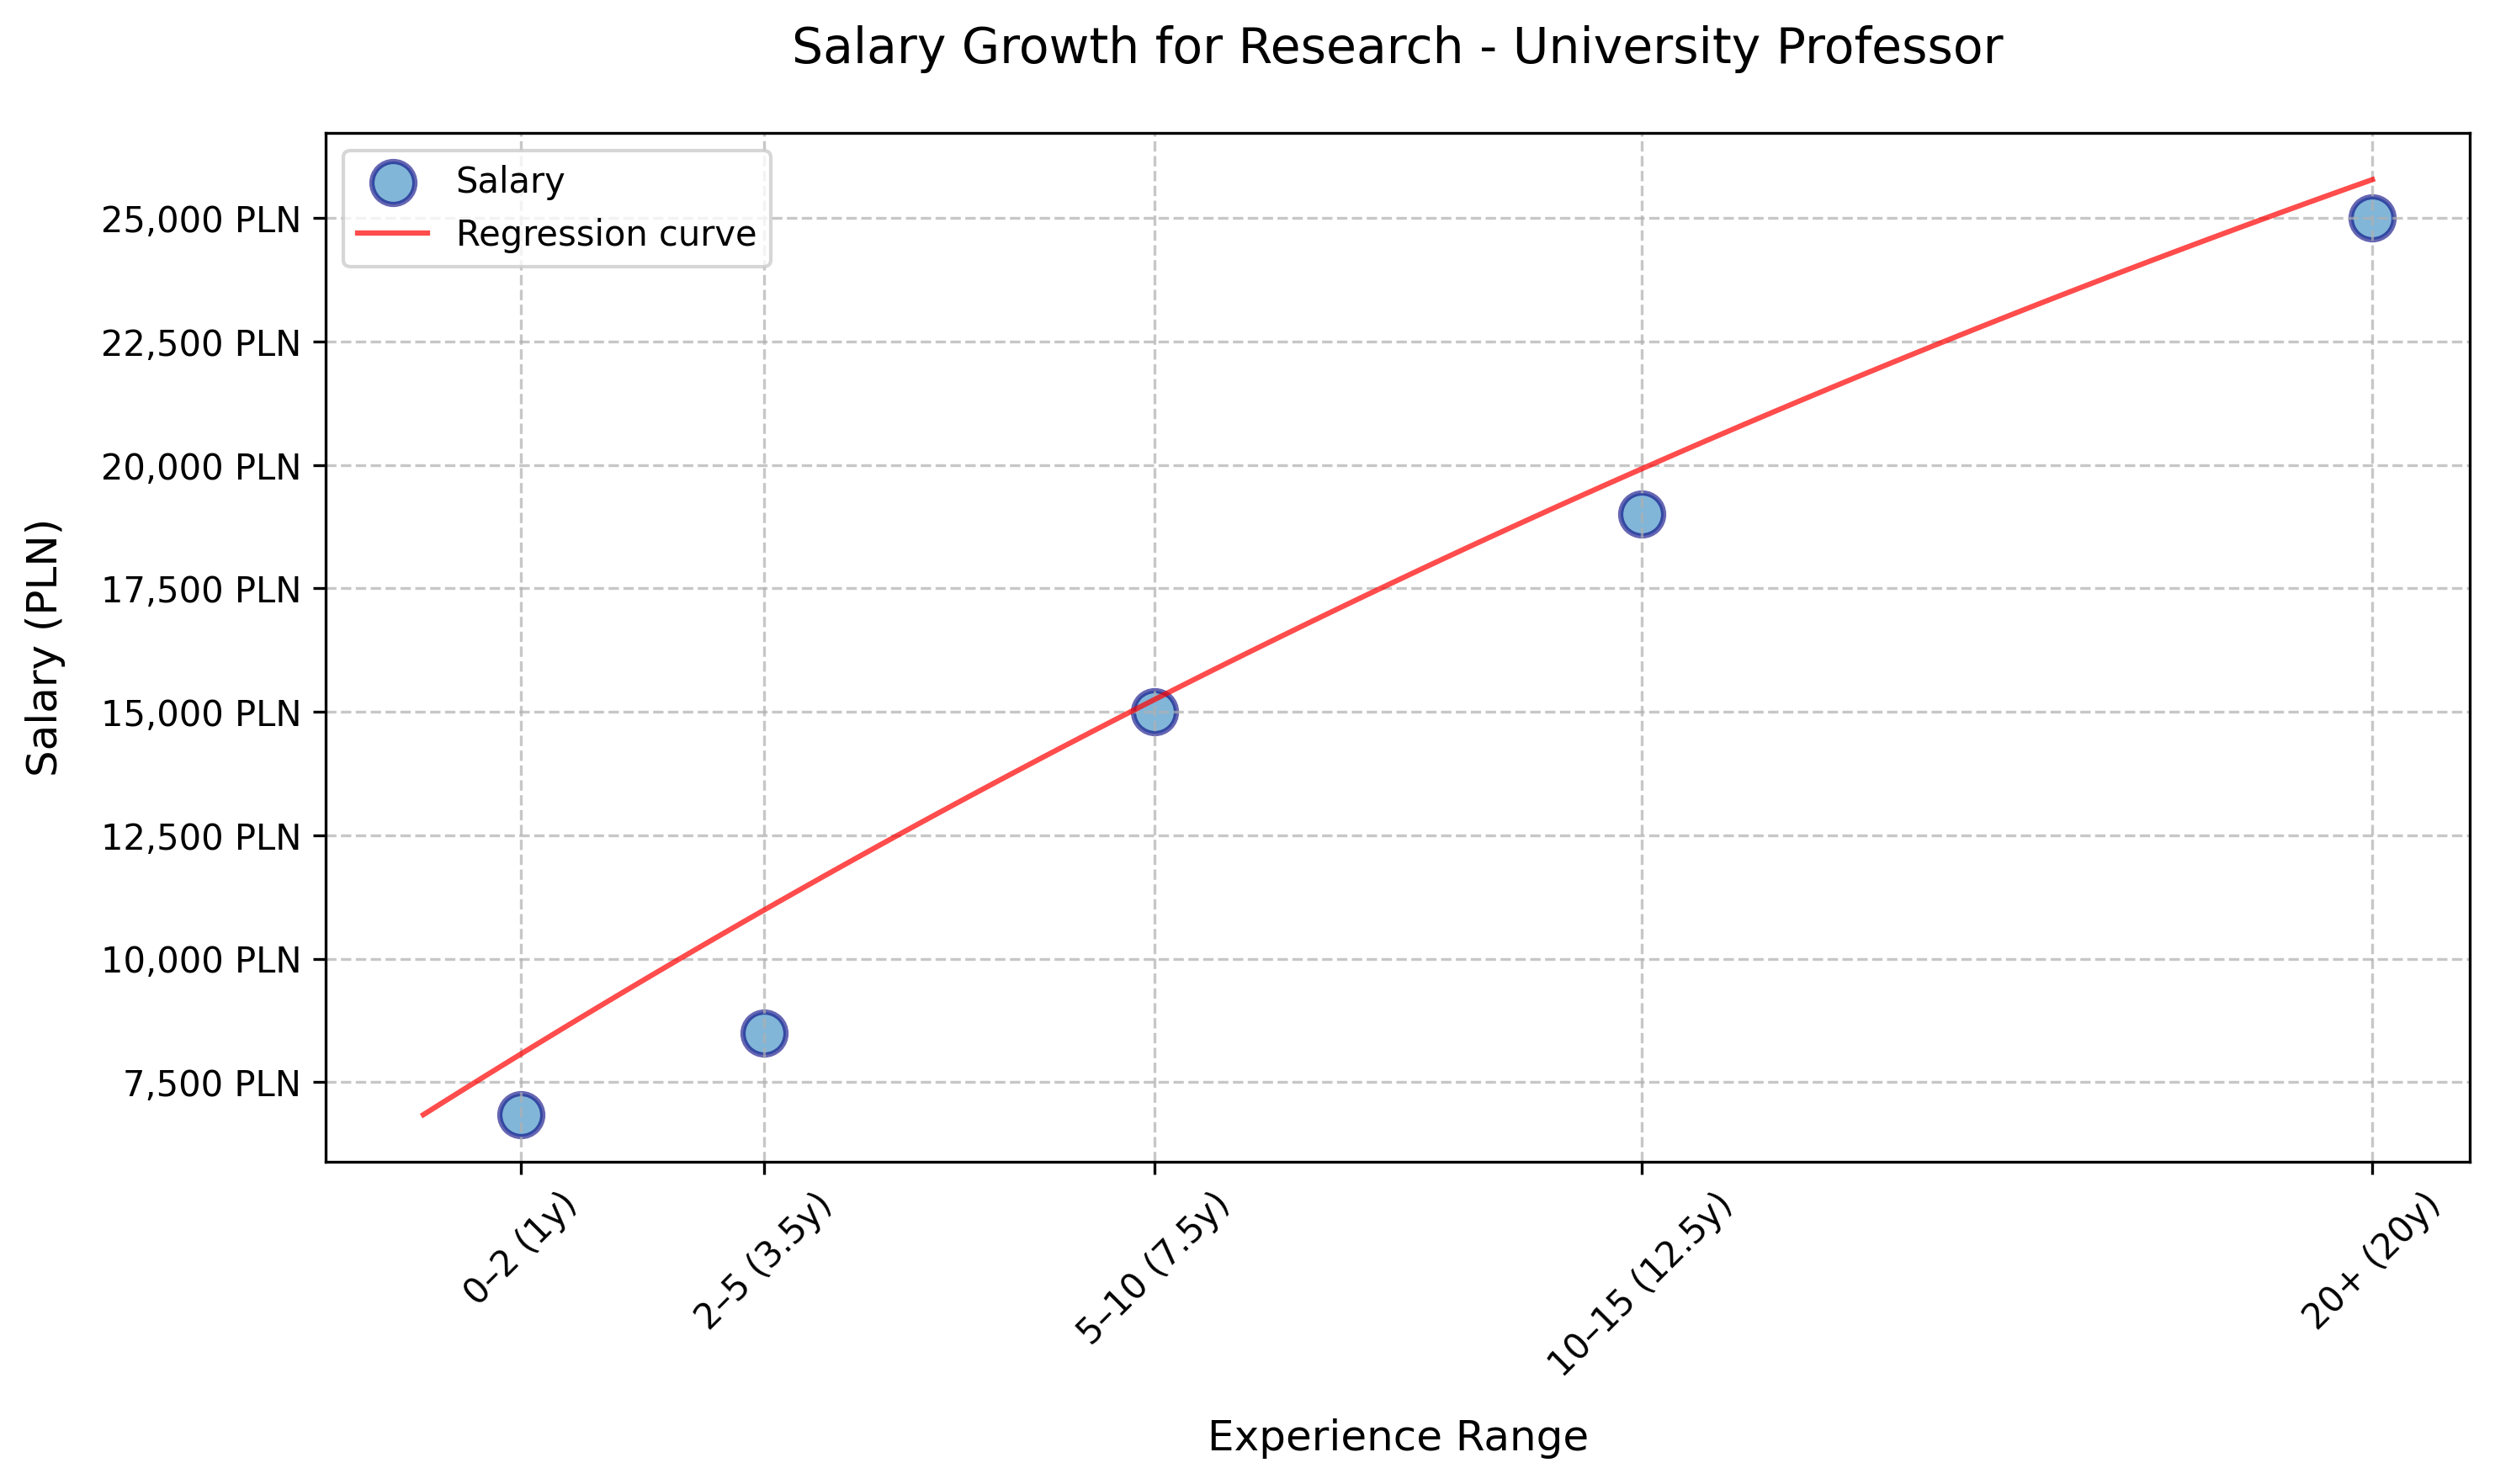
\includegraphics[width=0.45\linewidth]{img/salary_progression4} \\
    \pause
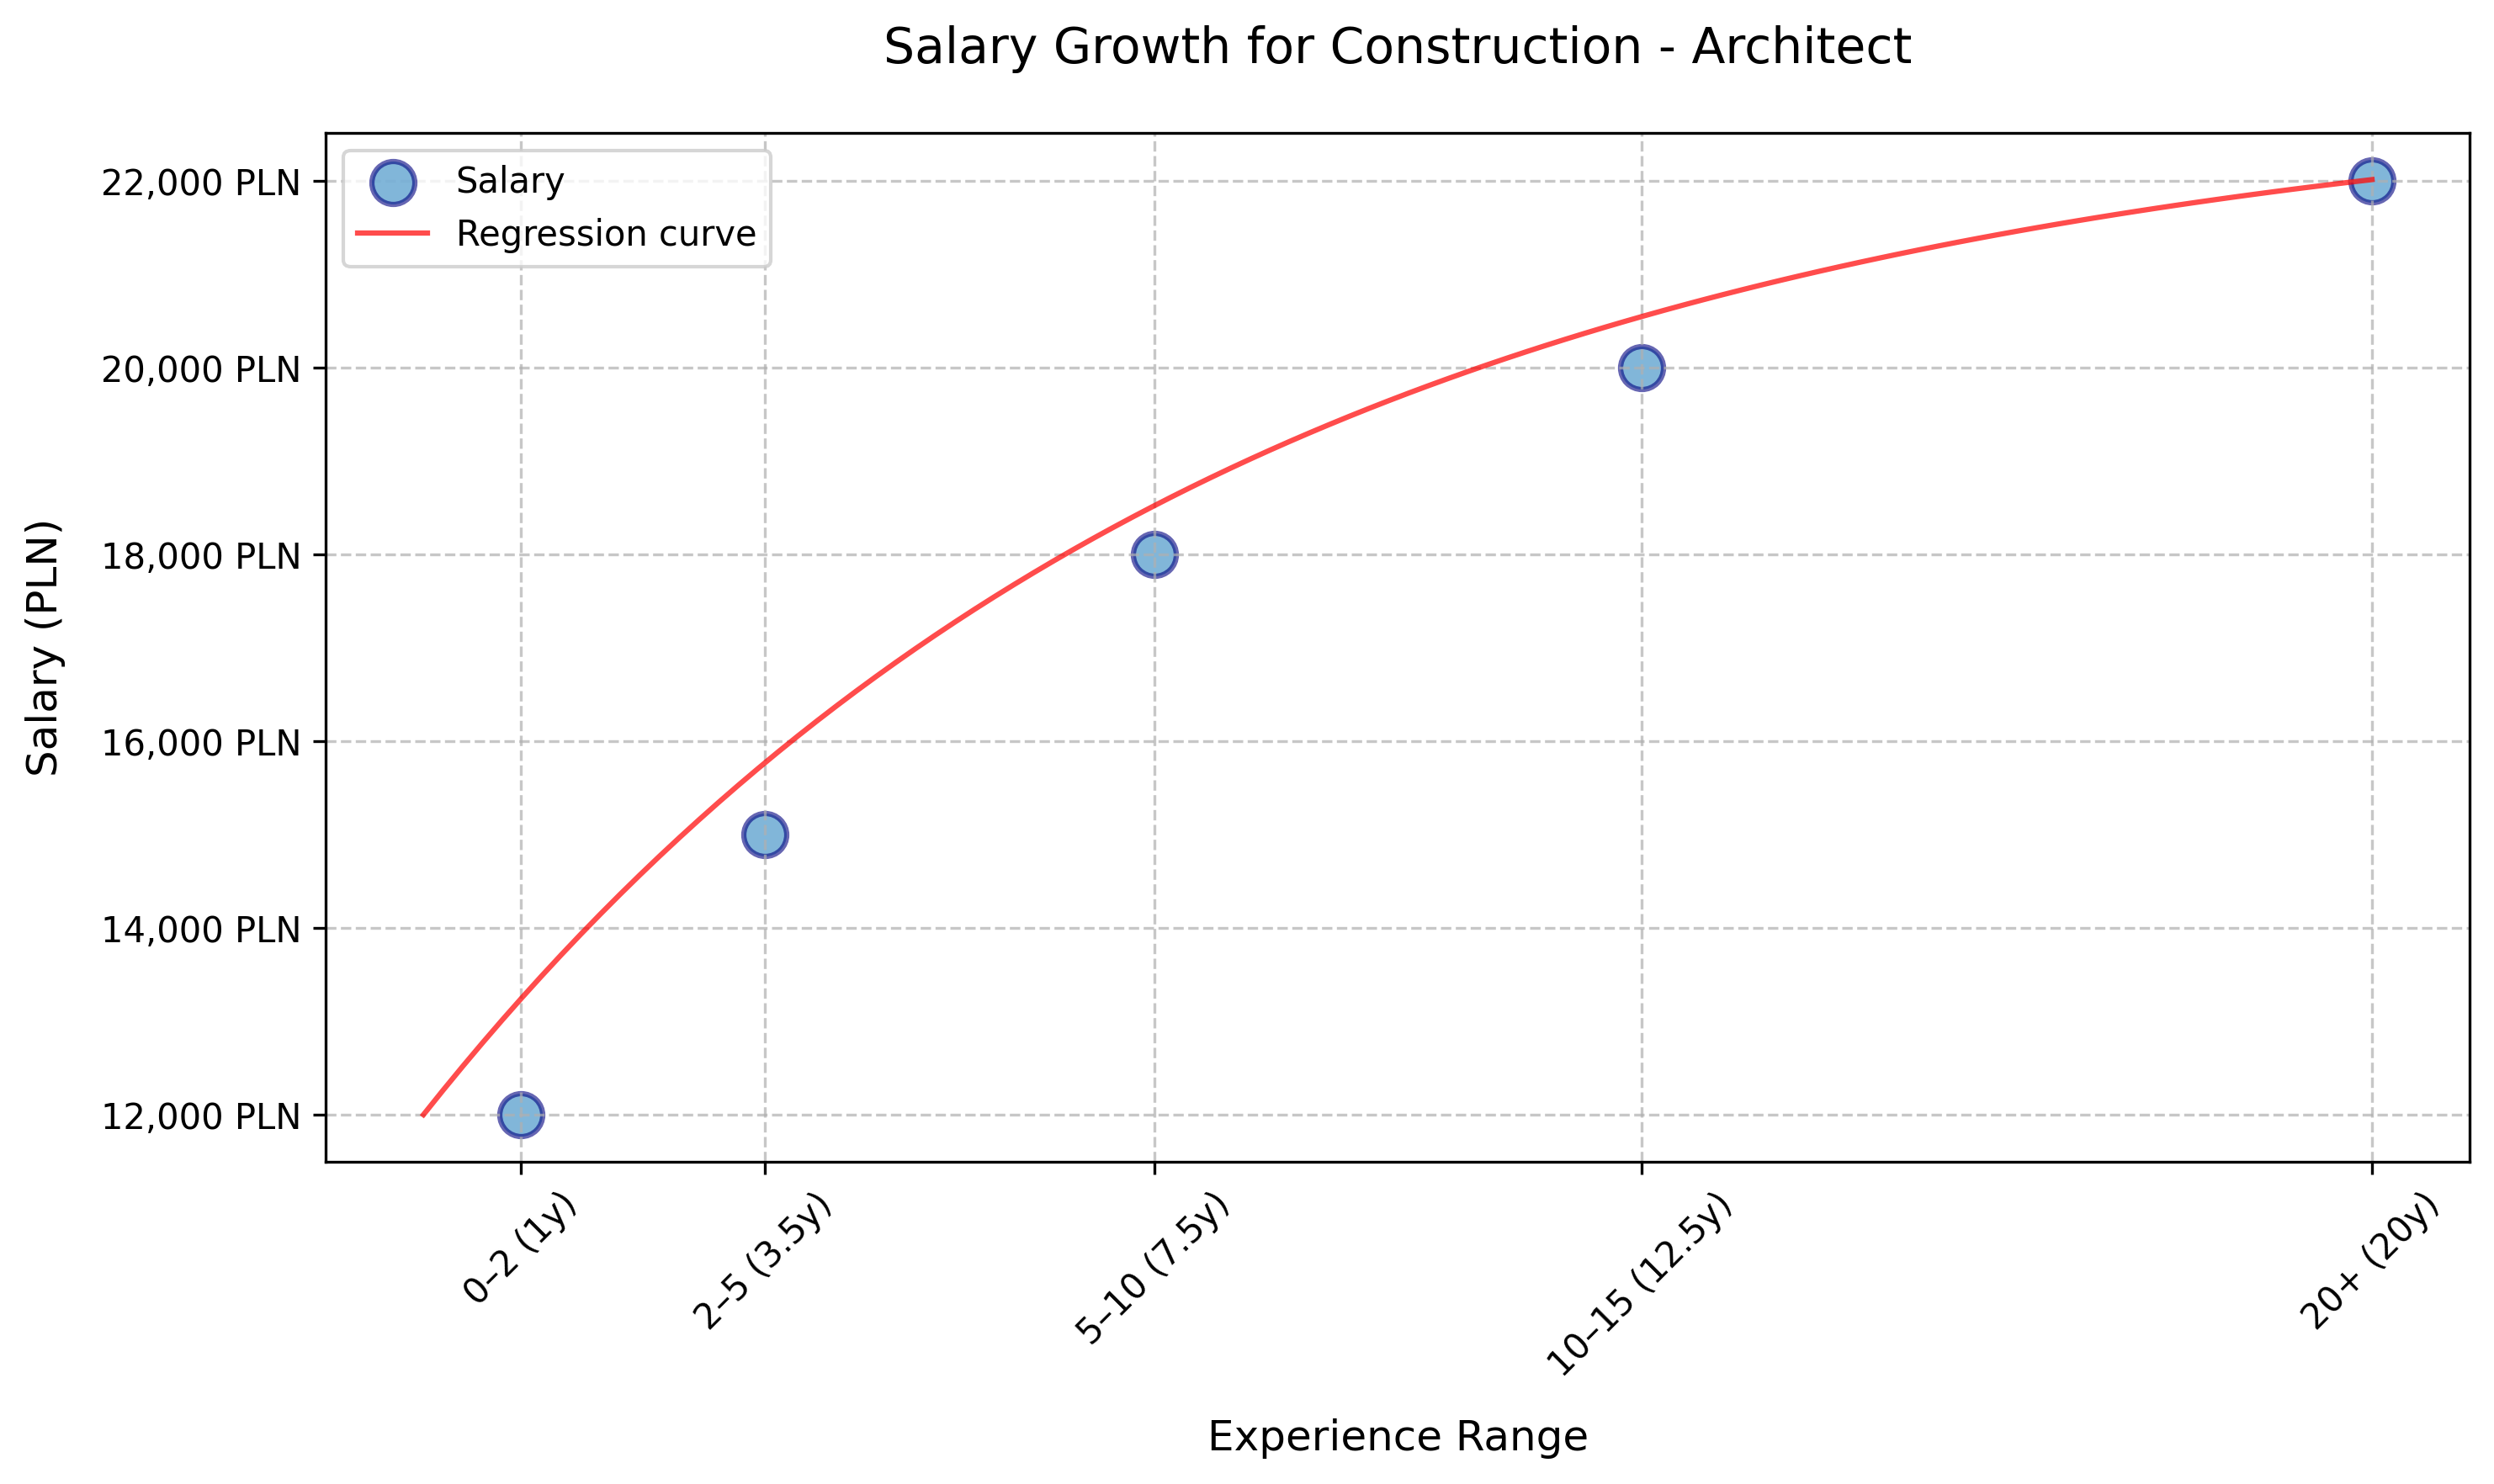
\includegraphics[width=0.45\linewidth]{img/salary_progression6} &
    \pause
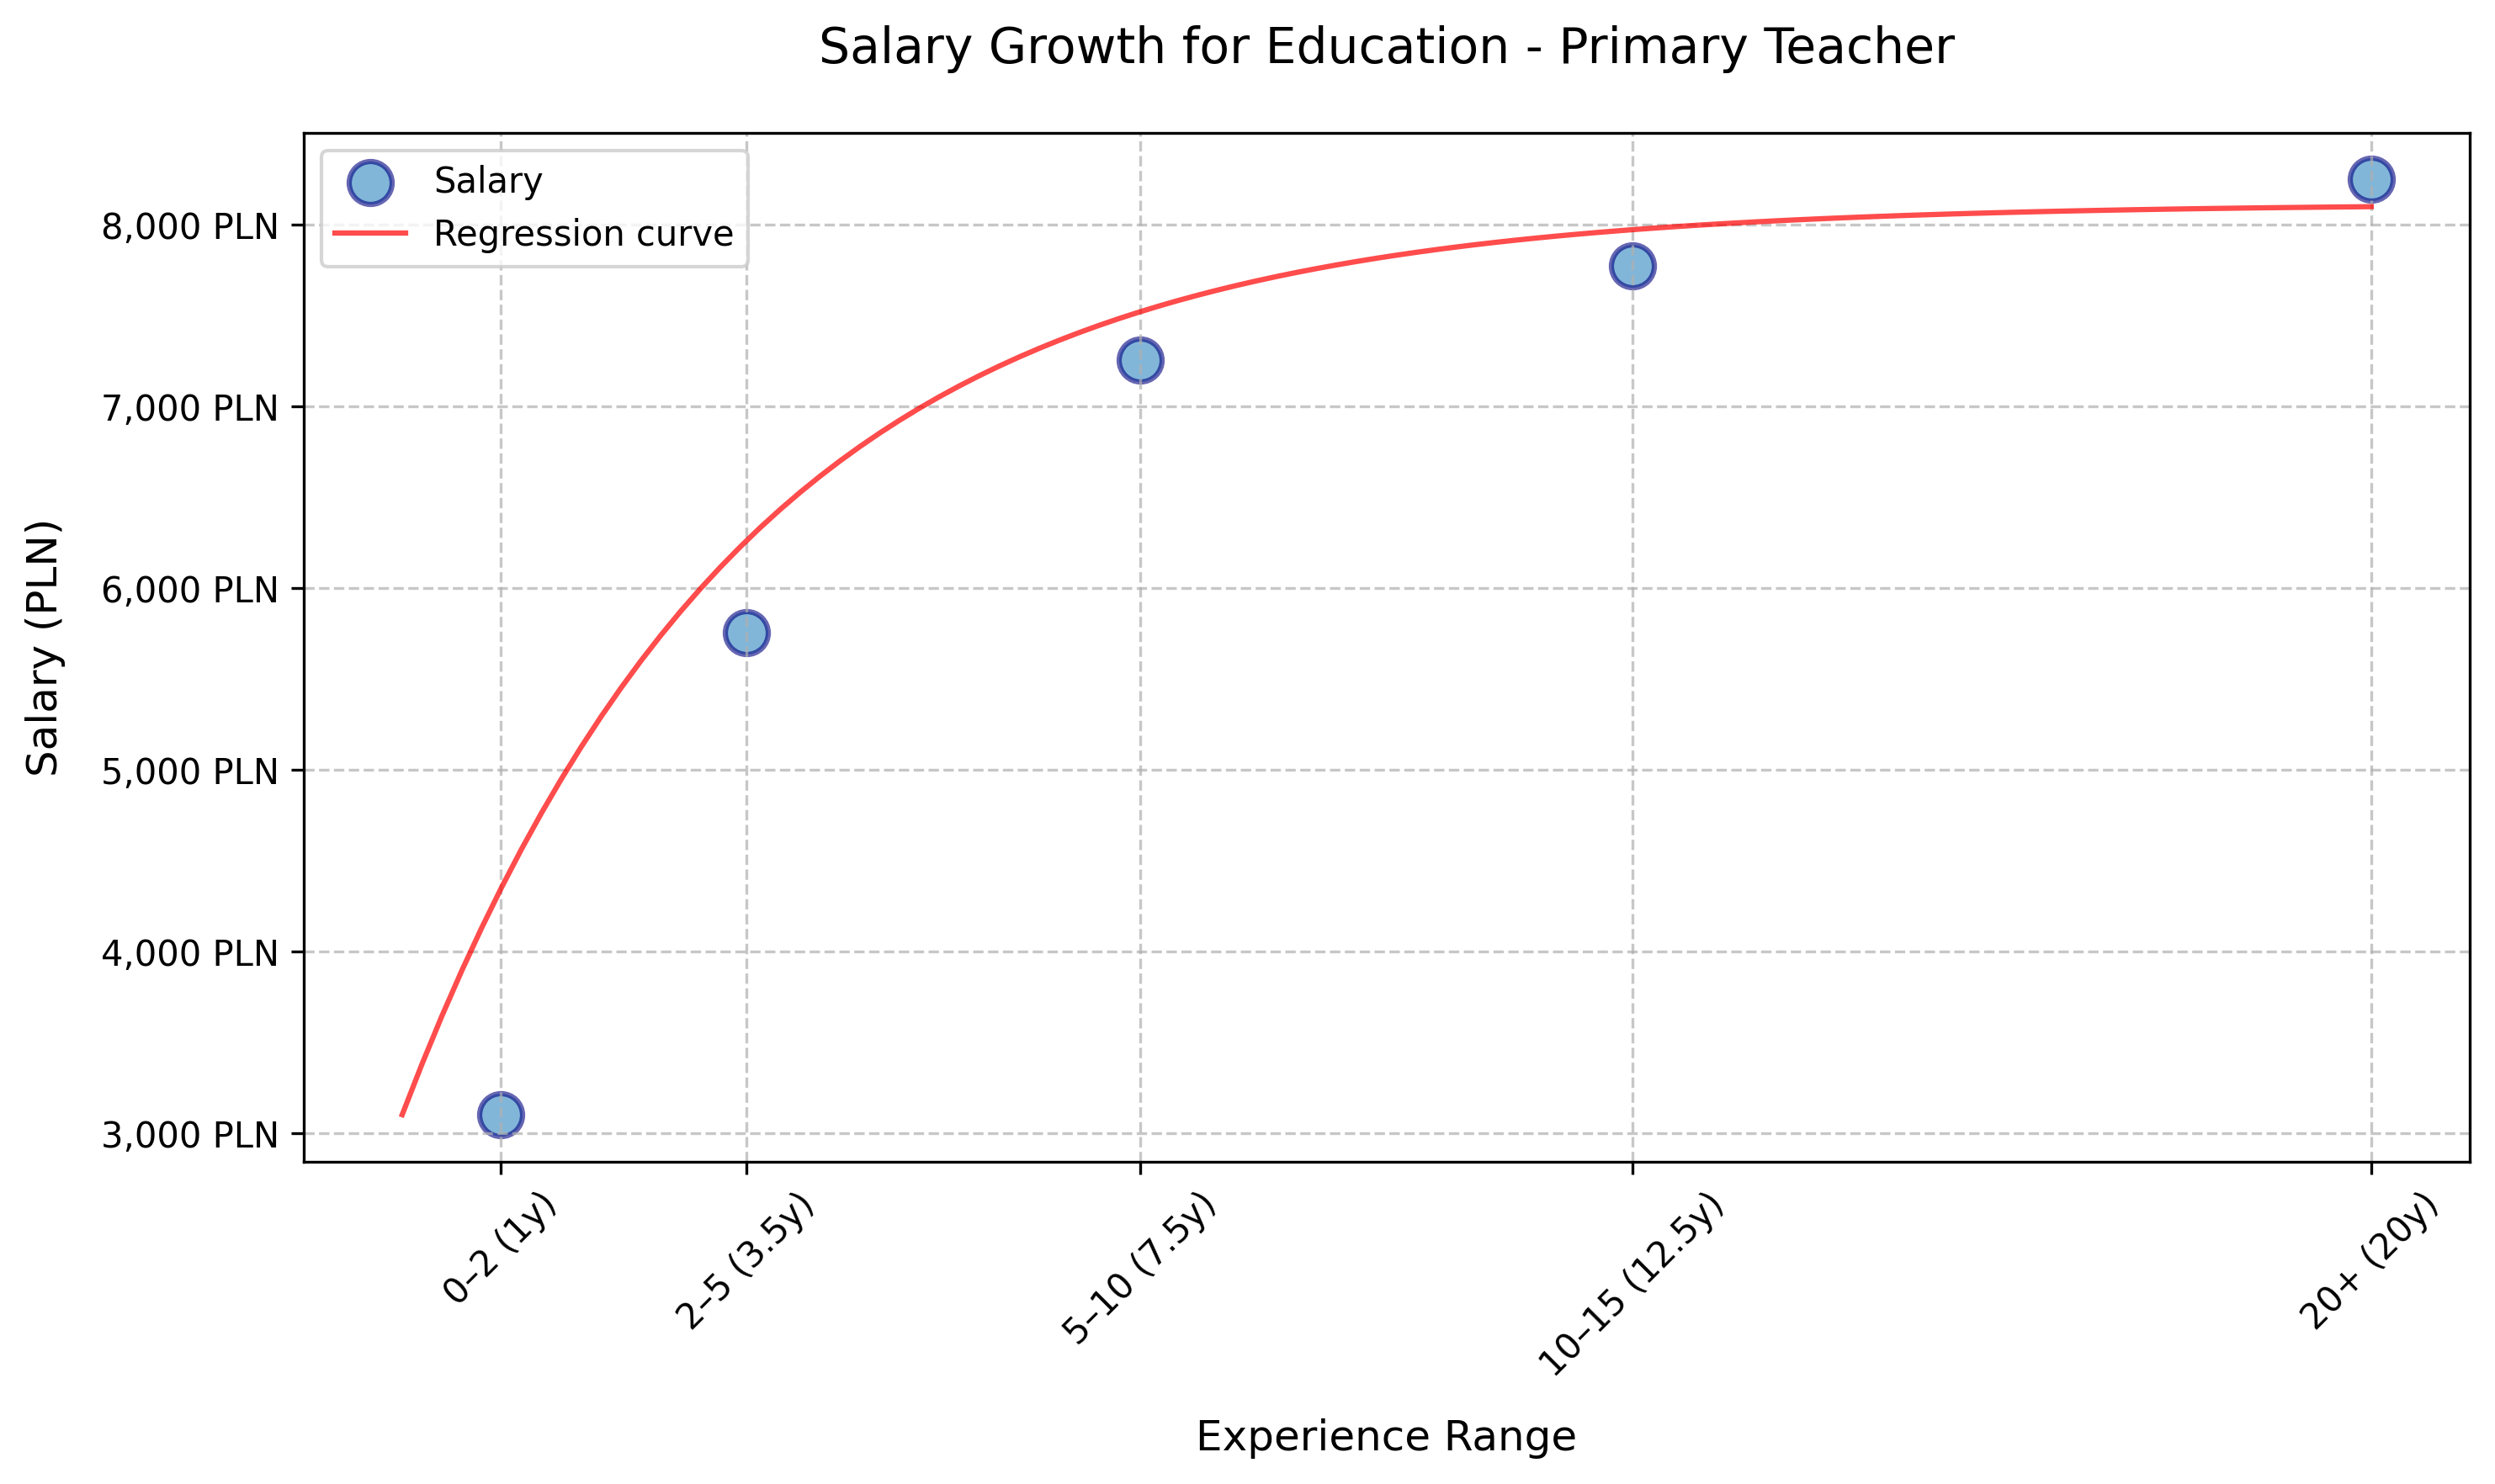
\includegraphics[width=0.45\linewidth]{img/salary_progression7}
\end{tabular}
\end{frame}

\begin{frame}[t]{LLMs and RAG}{Classification}
    \textbf{Using the Gemini API, we can assign any occupation to one of our pre‑trained models.}
    \\
    \pause
    \brand{With Retrieval‑Augmented Generation (RAG)
    we retrieve the current starting (junior) market rate for the given industry}
    \\
    \pause
    \highlight{By adding a model of macroeconomic factors such as inflation and GDP growth,
    we can credibly estimate the user’s entire financial history --- both past and future!}
\end{frame}
